\documentclass[paper=letter, fontsize=12pt]{article}
\usepackage{geometry}
\geometry{margin=1in}
\usepackage{graphicx}
\graphicspath{{images/}}
\usepackage{amssymb}
\usepackage{enumitem}
\usepackage{multirow}
\usepackage{longtable}

%opening
\title{Compsci 571 HW2}
\author{Yilin Gao (yg95)}

\begin{document}

\maketitle
\section{Classifier for Basketball Courts}

\begin{enumerate}[label=(\alph*)]
	% 1a
	\item When running Perceptron algorithm on the dataset, it takes 7 iterations (updates) to converge. The decision boundary is $f(x_1, x_2) = -1.05 * x_1 + 1.1 * x_2$. Because after it converges, all training points are correctly classified, the error rate is 0.
	
	Assume another linear classifier that goes through origin and achieves the same training error rate (0) as the perceptron classifier is $f(x_1, x_2) = w_1 * x_1 + w_2 * x_2$. Set $f(x_1, x_2) = 0$, we get the slope of the boundary is $-\frac{w_1}{w_2}$. From the plot of training data, we know that the boundary should go above point $[0.85, 0.80]$, and go below point $[0.85, 0.95]$. So $\frac{0.80}{0.85} < -\frac{w_1}{w_2} < \frac{0.95}{0.85}$. If we set $w_2 = 1$, we get $ -1.12< w_1 < -0.94$.
	
	The plot of observed data, the perceptron decision boundary (the light blue line), and all other linear boundaries that achieve the same training error (the yellow area) is:
	
	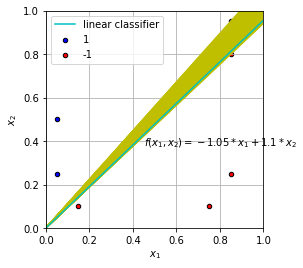
\includegraphics[scale=0.6]{q1a.png}
	
	%1b
	\item The fully-grown decision tree using Gini index as splitting criterion on the observed data is:
	
	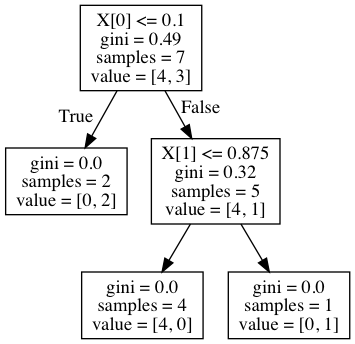
\includegraphics[scale=0.5]{q1b_tree.png}
	
	Because all training points are correctly classified by this tree, its training error is 0.
	
	Assume another decision tree with same training error (0) splits on the same feature order but different splitting threshold ($v_1$ for $x_1$ and $v_2$ for $x_2$). Then the threshold of the first split on $x_1$ should be able to separate points $[0.05, 0.25], [0.05, 0.5]$ (+1) with $[0.15, 0.1]$ (-1). So $v_1$ should be $\in (0.05, 0.15)$. The threshold of the second split on $x_2$ should be able to separate points $[0.85, 0.8]$ (-1) with $[0.85, 0.95]$ (+1). So $v_2$ should be $\in (0.8, 0.95)$.
	
	The plot of observed data, and the calculated decision boundary is:
	
	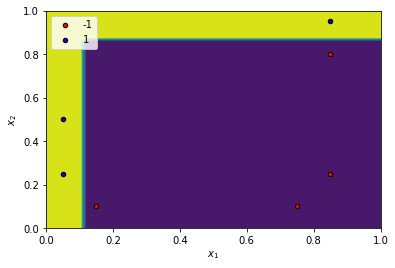
\includegraphics[scale=0.6]{q1b1.png}
	
	The plot of observed data, the calculated decision boundary, and all other decision boundaries that achieve the same training area (the red area) is:
	
	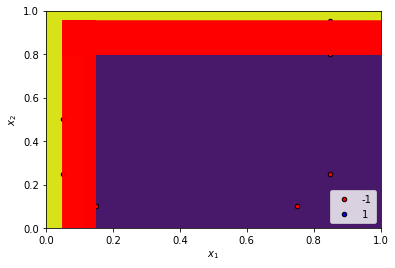
\includegraphics[scale=0.6]{q1b2.png}
	
	%1c
	\item 	Suppose the real optimal linear classifier that passes through the origin is $f(x_1, x_2) = w_1 * x_1 + w_2 * x_2$, such that it is able to minimize $R^{true}(f)$.
	
	\begin{equation}
	T = R^{true}(f) = \mathbb{E}_{(\mathbf{x}, y) \sim D}l(f(\mathbf{x}), y) = \mathbb{E}_{(\mathbf{x}, y) \sim D} \mathbf{1}_{[sign(f(\mathbf{x})) \neq y]}
	\end{equation}
	\begin{equation}
	= \mathbf{P}(sign(f(\mathbf{x})) \neq y)
	\end{equation}
	\begin{equation}
	= \mathbf{P}(y = 1, f(\mathbf{x}) \leq 0) + \mathbf{P}(y = -1, f(\mathbf{x}) \geq 0)
	\end{equation}
	\begin{equation}
	= \mathbf{P}(w_1  x_1 + w_2 x_2 \leq 0, 0 \leq x_1 \leq 1, \sqrt{x_1} \leq x_2 \leq 1) 
		+ \mathbf{P}(w_1 x_1 + w_2 x_2 \geq 0,  0 \leq x_1 \leq 1, 0 \leq x_2 \leq \sqrt{x_1})
	\end{equation}
	\begin{equation}
	= \mathbf{P}(x_2 \leq -\frac{w_1}{w_2} x_1,  0 \leq x_1 \leq 1, \sqrt{x_1} \leq x_2 \leq 1) 
	+  \mathbf{P}(x_2 \geq -\frac{w_1}{w_2} x_1, 0 \leq x_1 \leq 1, 0 \leq x_2 \leq \sqrt{x_1})
	\end{equation}
	
	Step (2) is from the property of expectation on indicator function. 
	
	Assign $k = -\frac{w_1}{w_2}$, $k \in [0, \infty)$, equation (5) becomes:
	
	\begin{equation}
	= \mathbf{P}(x_2 \leq k x_1, 0 \leq x_1 \leq 1, \sqrt{x_1} \leq x_2 \leq 1)
	+ \mathbf{P}(x_2 \geq k x_1, 0 \leq x_1 \leq 1, 0 \leq x_2 \leq \sqrt{x_1}) 
	\end{equation}
	
	So we need to find the optimized $k$ that minimizes $R^{true}(f)$, or equivalently equation (6).
	
	Because $(x_1, x_2)$ follow a uniform distribution, the 2 probability values in equation (6) are just areas formed by the border lines. We could use integration to compute them. (Here I use Python packages to compute the optimized values, see code for details.)
	
	If $k \in [0, 1]$, local optimized $k' = 1$ minimizes $T' =\frac{\pi}{4} - \frac{1}{2}$.
	
	If $k \in (1, \infty)$, local optimized $k'' = 1.4142$, and $T'' = 0.09763107$.
	
	So the global optimized $k^* = k'' = 1.4142$, the optimal linear classifier that passes through the origin is $\mathbf{f(x_1, x_2) = -1.4142 * x_1 + 1 * x_2 = 0}$, and the corresponding minimal $R^{true}(f) = 0.09763107$.
	
	This solution \textbf{is not} among the solutions that achieved the same loss (0) in part (a).
	
	The plot of the decision boundary (blue line) on the basketball court is:
	
	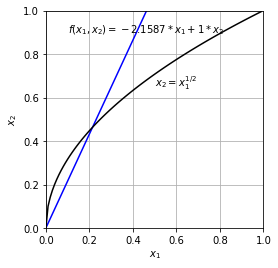
\includegraphics[scale=0.6]{q1c.png}
	
	%1d
	\item 
	\begin{equation}
	T = R^{true}(f) = \mathbf{P}(f(\mathbf{x}) \leq 0,  y = 1) + \mathbf{P}(f(\mathbf{x}) \geq 0,  y = -1)
	\end{equation}
	
	For tree 1 which starts splitting on $X_1$, there are 4 different conditions regarding $s_1, s_2, s_3$:
	
	If $0 \leq s_2 < \sqrt{s_1}$ and $\sqrt{s_1} < s_3 \leq 1$, $\min_{s_1, s_2, s_3} T = \int_{0}^{s_2^2} (s_2 - \sqrt{x}) dx + \int_{s_2^2}^{s_1} (\sqrt{x} - s_2) dx + \int_{s_1}^{s_3^2} (s_3 - \sqrt{x}) dx + \int_{s_3^2}^{1} (\sqrt{x} - s_3) dx$
	
	If $0 \leq s_2 < \sqrt{s_1}$ and $0 \leq s_3 \leq \sqrt{s_1}$, $\min_{s_1, s_2, s_3} T = \int_{0}^{s_2^2} (s_2 - \sqrt{x}) dx + \int_{s_2^2}^{s_1} (\sqrt{x} - s_2) dx + \int_{s_1}^{1} (\sqrt{x} - s_3) dx = \min_{s_1, s_2, s_3 = \sqrt{s_1}} (\int_{0}^{s_2^2} (s_2 - \sqrt{x}) dx + \int_{s_2^2}^{s_1} (\sqrt{x} - s_2) dx + \int_{s_1}^{1} (\sqrt{x} - \sqrt{s_1} dx)$
	
	If $\sqrt{s_1} \leq s_2 \leq 1$ and $\sqrt{s_1} < s_3 \leq 1$, $\min_{s_1, s_2, s_3} T = \int_{0}^{s_1} (s_2 - \sqrt{x}) dx + \int_{s_1}^{s_3^2} (s_3 - \sqrt{x}) dx + \int_{s_3^2}^{1} (\sqrt{x} - s_3) dx = \min_{s_1, s_2 = \sqrt{s_1}, s_3} (\int_{0}^{s_1} (\sqrt{s_1} - \sqrt{x}) dx + \int_{s_1}^{s_3^2} (s_3 - \sqrt{x}) dx + \int_{s_3^2}^{1} (\sqrt{x} - s_3) dx)$
	
	If $\sqrt{s_1} \leq s_2 \leq 1$ and $0 \leq s_3 \leq \sqrt{s_1}$, $\min_{s_1, s_2, s_3} T = \int_{0}^{s_1} (s_2 - \sqrt{x}) dx + \int_{s_1}^{1} (\sqrt{x} - s_3) dx = \min_{s_1, s_2 = \sqrt{s_1}, s_3 = \sqrt{s_1}} (\int_{0}^{s_1} (\sqrt{s_1} - \sqrt{x}) dx + \int_{s_1}^{1} (\sqrt{x} - \sqrt{s_1}) dx)$
	
	The global optimized solutions are $\mathbf{s_1 = 0.42677801, s_2 = 0.46194124, s_3 = 0.84462275}$ which gives minimal  $R^{true}(f) = \mathbf{0.1035845342551841}$. (See code for calculation details.)
	
	The real optimized tree decision boundary \textbf{is not} among those achieved in part (b).
	
	The plot of the decision boundary (blue line) on the basketball court is:
	
	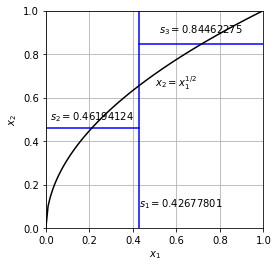
\includegraphics[scale=0.6]{q1d1.png}
	
	For the tree which starts splitting from $X_2$, there are also 4 different conditions regarding $s_1, s_2, s_3$:
	
	If $0 \leq s_2 < s_1^2$ and $s_1^2 < s_3 \leq 1$, $\min_{s_1, s_2, s_3} T = \int_{0}^{s_2} \sqrt{x} dx + \int_{s_2}^{s_1^2} (s_1 - \sqrt{x}) dx + \int_{s_1^2}^{s_3} (\sqrt{x} - s_1) dx + \int_{s_3}^{1} (1 - \sqrt{x}) dx$
	
	If $ s_1^2 \leq s_2 \leq 1$ and $s_1^2 < s_3 \leq 1$, $\min_{s_1, s_2 = s_1^2, s_3} T = \int_{0}^{s_1^2} \sqrt{x} dx + \int_{s_1^2}^{s_3} (\sqrt{x} - s_1) dx + \int_{s_3}^{1} (1 - \sqrt{x}) dx$
	
	If $0 \leq s_2 < s_1^2$ and $0 \leq s_3 \leq s_1^2$, $\min_{s_1, s_2, s_3 = s_1^2} T = \int_{0}^{s_2} \sqrt{x} dx + \int_{s_2}^{s_1^2} (s_1 - \sqrt{x}) dx + \int_{s_1^2}^{1} (1 - \sqrt{x}) dx$
	
	If $ s_1^2 \leq s_2 \leq 1$  and $0 \leq s_3 \leq s_1^2$, $\min_{s_1, s_2 = s_1^2, s_3 = s_1^2} T = \int_{0}^{s_1^2} \sqrt{x} dx + \int_{s_1^2}^{1} (1 - \sqrt{x}) dx$
	
	The global optimized solutions are $\mathbf{s_1 = 0.60762617, s_2 = 0.09230456, s_3 = 0.64611553}$ which gives minimal  $R^{true}(f) = \mathbf{0.11796176307566364}$. (See code for calculation details.)
	
	The real optimized tree decision boundary \textbf{is not} among those achieved in part (b).
	
	The plot of the decision boundary (blue line) on the basketball court is:
	
	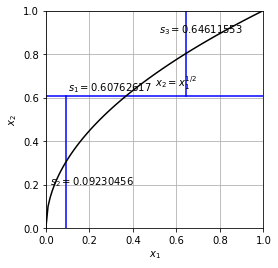
\includegraphics[scale=0.6]{q1d2.png}
	
	%1e
	\item Transform $x_2$ into $\mathbf{x_2^* = x_2^2}$. So now $x_1 \in [0, 1]$, $x_2^* \in [0, 1]$, and the true boundary for the 3-point line is $x_2^* = x_1$.
	
	Suppose the real optimal linear classifier that passes through the origin is $f(x_1, x_2^*) = w_1 x_1 + w_2^* x_2^*$.
	
	\begin{equation}
	T = R^{true}(f) =  \mathbf{P}(f(\mathbf{x^*}) \leq 0, y = 1) + \mathbf{P}(f(\mathbf{x^*}) \geq 0, y = -1) 
	\end{equation}
	\begin{equation}
	= \mathbf{P}(x_2^* \leq -\frac{w_1}{w_2^*} x_1, 0 \leq x_1 \leq 1, x_2^* \geq x_1) + \mathbf{P}(x_2^* \geq -\frac{w_1}{w_2^*} x_1, 0 \leq x_1 \leq 1, x_2^* \leq x_1) 
	\end{equation}
	
	And it is easy to find out that the optimal value of $\mathbf{-\frac{w_1}{w_2^*} = 1}$, the optimal linear classifier that passes through the origin is $\mathbf{f(x_1, x_2^*) = -x_1 + x_2^* = 0}$, and the corresponding minimal true error is \textbf{0}.
	
	%1f
	\item With the same transformation of $x_2$ as in part (e), a decision tree \textbf{cannot} achieve the same minimal true error (0) as the linear classifier in part (e). This is because the splitting boundary of decision tree can never be a line going through the origin.
	
	%1g
	\item For paint, assume the part inside paint ($0.5 \leq x_1 \leq 1$ and $0 \leq x_2 \leq 0.25$) has label $y = -1$ and the part outside paint has $y = 1$.
	 
	Same as in part (c), suppose the real optimal linear classifier that passes through the origin is $f(x_1, x_2) = w_1 x_1 + w_2 x_2$, such that it is able to minimize $R^{true}(f)$.
	
	\begin{equation}
	T = R^{true}(f) = \mathbf{P}(f(\mathbf{x}) \leq 0, y = 1) + \mathbf{P}(f(\mathbf{x}) \geq 0, y = -1)
	\end{equation}
	\begin{equation}
	= \mathbf{P}(x_2 \leq -\frac{w_1}{w_2} x_1, y = 1) +\mathbf{P}(x_2 \geq -\frac{w_1}{w_2} x_1, y = -1)
	\end{equation}
	
	Assign $k = -\frac{w_1}{w_2}$, $k \in [0, \infty)$,
	
	\begin{equation}
	=\mathbf{P}(x_2 \leq k x_1, y = 1) + \mathbf{P}(x_2 \geq k x_1, y = -1)
	\end{equation}
	
	If $k \in [\frac{1}{2}, \infty)$, local optimized $k' = \frac{1}{2}$ minimizes $T' = \frac{1}{8}$.
	
	If $k \in (\frac{1}{4}, \frac{1}{2})$, $min_{k} T = \int_{0}^{\frac{1}{2}} kx dx + \int_{\frac{1}{2}}^{\frac{1}{4k}} (\frac{1}{4} - kx) dx$. And the local optimized $k'' = 	0.35355341$ minimizes $T'' = 0.0517766952966372$.
	
	If $k \in [0, \frac{1}{4}]$, $min_{k} T = \int_{0}^{\frac{1}{2}} kx dx + \int_{\frac{1}{2}}^{1}(\frac{1}{4} - kx) dx = 0.0625$ when $k = \frac{1}{4}$.

	So in conclusion, the global optimized $-\frac{w_1}{w_2} = k = \mathbf{0.35355341}$, the optimal linear classifier that passes through the origin is $\mathbf{f(x_1, x_2) = -0.35355341 x_1 + x_2 = 0}$, and the corresponding minimal true error rate $R^{true}(f) = \mathbf{0.0517766952966372}$.
	
	The plot of the decision boundary on the basketball court is:
	
	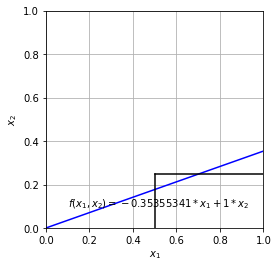
\includegraphics[scale=0.6]{q1g.png}
	
	%1h
	\item The optimal depth 2 decision tree will split on $x_1 = m$ and $x_2 = n$. And $f(\mathbf{x}) = -1$ if $m \leq x_1 \leq 1$ and $0 \leq x_2 \leq n$, $f(\mathbf{x}) = 1$ otherwise.
	
	\begin{equation}
	T = R^{true}(f) =  \mathbf{P}(f(\mathbf{x}) \leq 0, y = 1) + \mathbf{P}(f(\mathbf{x}) \geq 0, y = -1)
	\end{equation}
	
	It's easy to find out that when $\mathbf{m = \frac{1}{2}}$ and $\mathbf{n = \frac{1}{4}}$, both $\mathbf{P}(f(\mathbf{x}) \leq 0, y = 1)$ and $\mathbf{P}(f(\mathbf{x}) \geq 0, y = -1) $ are equal to 0, and $T$ achieves its minimal value \textbf{0}. The depth 2 decision tree looks like:
	
	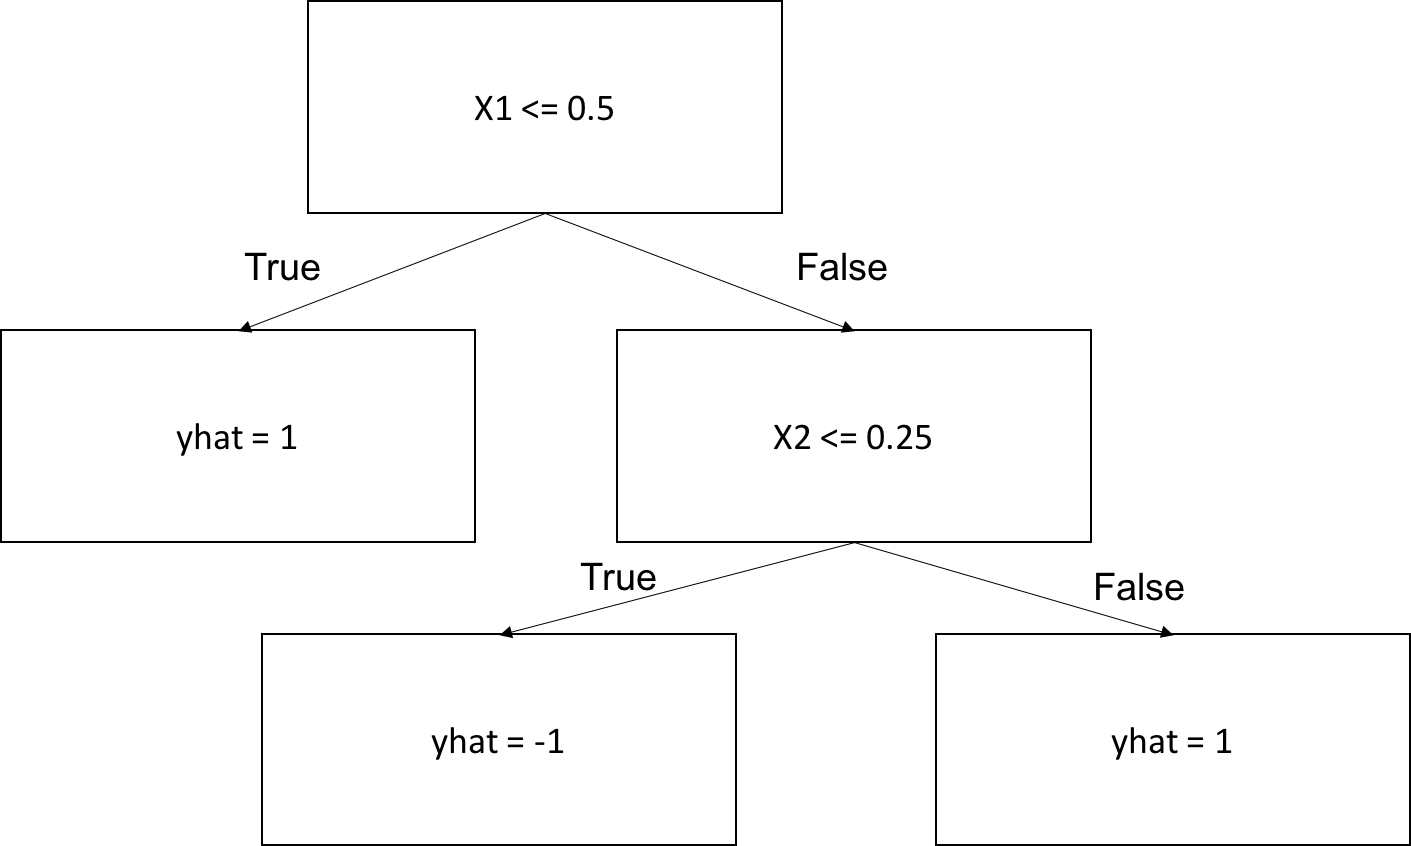
\includegraphics[scale=0.3]{q1h.png}
	
\end{enumerate}

\section{Variable Importance for Trees and Random Forests}

\begin{enumerate}[label=(\alph*)]
	\item 
	\begin{enumerate}[label=(\roman*)]
		\item 
		The decision stump based on the \textbf{best split} (for each node, split on the variable with largest reduction in Gini Index) is:
		
		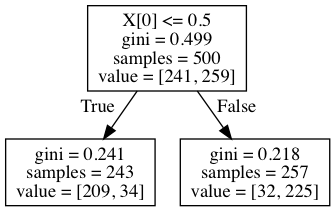
\includegraphics[scale=0.6]{tree_best_split.png}
		
		At root it splits on independent variable $X_1$ (shown as $X[0]$ in picture) on the threshold $s_1 = 0.5$.
		
		The decision stump based on the \textbf{best surrogate split} is:
		
		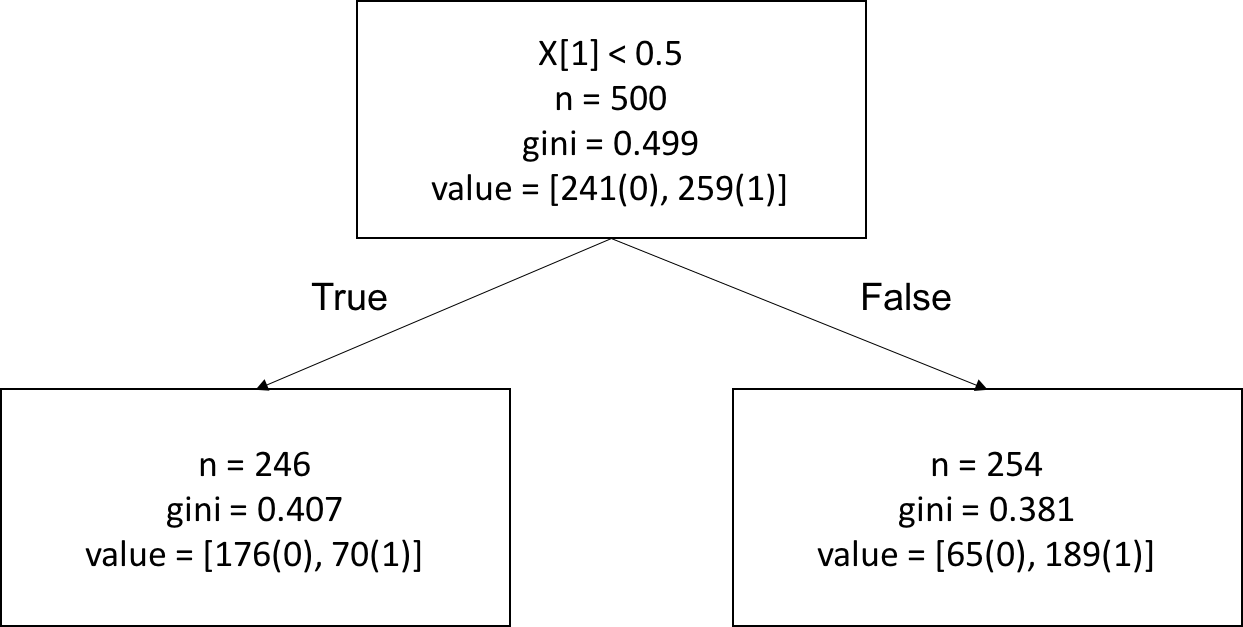
\includegraphics[scale=0.4]{tree_best_surrogate_split.png}
		
		This tree is generated by choosing the best surrogate split on the root (by comparing the predictive similarity measure on variables $X_2$, $X_3$, $X_4$ and $X_5$). At root it chooses $X_2$ (shown as $X[1]$ in picture) as the best surrogate split, with threshold 0.5 (actually this value doesn't really matter).
		
		\item Variable importance measures from equation (2) are:
		
		\begin{center}
			\begin{tabular}{|c|c|}
				\hline
				$X_1$ & $0.2703$ \\ \hline
				$X_2$ & NA \\ \hline
				$X_3$ & NA \\ \hline
				$X_4$ & NA \\ \hline
				$X_5$ & NA \\ \hline
			\end{tabular}
		\end{center}
			
		Variable importance measures from equation (3) are:
		
		\begin{center}
			\begin{tabular}{|c|c|}
				\hline
				$X_1$ & $0.2703$ \\ \hline
				$X_2$ & $0.1056$ \\ \hline
				$X_3$ & NA \\ \hline
				$X_4$ & NA \\ \hline
				$X_5$ & NA \\ \hline
			\end{tabular}
		\end{center}
	
		(See code for calculation process)
	
		If we only refer to the variable importance measures from equation (2), we can only say variable $X_1$ is the known most important variable among the five, but not sure if any other variables has similar importance as it.
		
		With the variable importance measures from equation (3), we could see comparing variable $X_1$ and its most close substitute/surrogate $X_2$, $X_1$ is still more important than $X_2$. So we could suggest with more confidence that $X_1$ is more important than others.
		
		\item 
		The mean squares error of predictions on the test data from the decision stump based on the best split is 0.1.
		
		The mean squares error of predictions on the test data from the decision stump based on the best surrogate split is 0.27. 
		
		(see code for calculation process)
		
	\end{enumerate}

	\item 
	For all following random forests in (b) and (c), I set the Python numpy random seed to 111.
	
	\begin{enumerate}[label=(\roman*)]
		\item The table for best split variable and best surrogate variable for each $K$ is:
		
		(Note that when $K = 1$ there are only 999 trees in the forest, because there is one potential tree generating negative reduction in Gini index, and this tree is dropped. And whether this happens or not depends on the bootstrap training sample selected for each tree.)
		
		\begin{center}
			\begin{longtable}{|c|c|c|c|}
				\hline
				$K$ & variable & time as best split variable  & time as best surrogate variable \\ \hline
				\multirow{5}{1em}{1} & $X_1$ & 215 & 0 \\ 
				& $X_2$ & 203 & 0\\
				& $X_3$ & 186 & 0\\
				& $X_4$ & 192 & 0\\
				& $X_5$ & 203 & 0\\
				\hline
				\multirow{5}{1em}{2} & $X_1$ & 399 & 0\\ 
				& $X_2$ & 312 & 106\\
				& $X_3$ & 119 & 291\\
				& $X_4$ & 116 & 268\\
				& $X_5$ & 54 & 335\\
				\hline
				\multirow{5}{1em}{3} & $X_1$ & 585 & 0 \\ 
				& $X_2$ & 321 & 291\\
				& $X_3$ & 48 & 288\\
				& $X_4$ & 39 & 146\\
				& $X_5$ & 7 & 275\\
				\hline
				\multirow{5}{1em}{4} & $X_1$ & 788 & 0\\ 
				& $X_2$ & 212 & 582\\
				& $X_3$ & 0 & 168\\
				& $X_4$ & 0 & 22\\
				& $X_5$ & 0 & 228\\
				\hline
				\multirow{5}{1em}{5} & $X_1$ & 1000 & 0\\ 
				& $X_2$ & 0 & 1000\\
				& $X_3$ & 0 & 0\\
				& $X_4$ & 0 & 0\\
				& $X_5$ & 0 & 0\\
				\hline
			\end{longtable}
		\end{center}	
	
		First of all, we need to make clear the implication of different values of $K$. When $K$ is smaller (like 1), variables are given more equal opportunities to become the best split variable. When $K$ is larger (like 5), the competition between variables to become the best split gets more fierce, and important variables are more likely to win out as the best split.
	
		So according to the frequency of best split variables, $X_1$ is selected as the best split variable more as $K$ increases. So this suggests variable $X_1$ is more important than others.
		
		And according to the frequency of best surrogate split variables, $X_2$ is selected more as $K$ increases. So this suggests while $X_1$ is important, the importance of $X_2$ could have been masked by that of $X_1$. So we also need to consider the importance of $X_2$.
		
		\item The variable importance according to equations (5) and (6) for each $K$ is:
		
		\begin{longtable}{|c|c|c|c|}
			\hline
			$K$ & variable & variable importance (5) & variable importance (6) \\ \hline
			\multirow{5}{1em}{1} & $X_1$ & 0.269419 & 0.370326 \\ 
			& $X_2$ & 0.105597 & 0.228473 \\
			& $X_3$ & 0.000926 & -0.024192 \\
			& $X_4$ & 0.000908 & 0.009479 \\
			& $X_5$ & 0.000405 & -0.033300 \\
			\hline
			\multirow{5}{1em}{2} & $X_1$ & 0.270229 & 0.364712 \\ 
			& $X_2$ & 0.106150 & 0.225641 \\
			& $X_3$ & 0.001206 & -0.019158 \\
			& $X_4$ & 0.001266 & -0.018274 \\
			& $X_5$ & 0.000684 & -0.040000 \\
			\hline
			\multirow{5}{1em}{3} & $X_1$ & 0.270640 & 0.363863 \\ 
			& $X_2$ & 0.105558 & 0.227726 \\
			& $X_3$ & 0.001323 & -0.021665 \\
			& $X_4$ & 0.001396 & -0.023588 \\
			& $X_5$ & 0.001013 & -0.034284 \\
			\hline
			\multirow{5}{1em}{4} & $X_1$ & 0.270346 & 0.364391 \\ 
			& $X_2$ & 0.105903 & 0.230000 \\
			& $X_3$ & NaN & NaN \\
			& $X_4$ & NaN & NaN \\
			& $X_5$ & NaN & NaN \\
			\hline
			\multirow{5}{1em}{5} & $X_1$ & 0.270640 & 0.36388 \\ 
			& $X_2$ & NaN & NaN \\
			& $X_3$ & NaN & NaN \\
			& $X_4$ & NaN & NaN \\
			& $X_5$ & NaN & NaN \\
			\hline
		\end{longtable}
	
		As these are all average variable importance over all trees, importance of each variable under different values of $K$ shouldn't show significant difference, which is consistent with the empirical results. And if some variables are never selected as the best split variable, they won't have either variable importance (5) or (6).
		
		Both variable importance (5) and (6) for all the $K = \{1, 2, 3, 4, 5\}$ suggest variable $X_1$ is the most important one, and $X_2$ is the second important one. And the importance of $X_1$ and $X_2$ are much higher that that of other variables.
		
		As $K$ increase, the problem of masking is exaggerated. When $K = 5$, only variable $X_1$ is selected as the best split, thus only its importance can be computed. We can never know the importance of other variables.
		
		But when $K$ is small, each variable is given more opportunities to be selected as the best split. And when a variable is selected as the best split, it is able to demonstrate its importance. So the results of $K = 1$ could lessen the impact of masking.
		
		\item The mean squares loss on the test data using the random forest with 2 methods:
		
		\begin{center}
			\begin{tabular}{|c|c|c|}
				\hline
				$K$ & method 1 & method 2 \\ \hline
				1 & 0.17  & 0.358240 \\ \hline
				2 & 0.15 & 0.262910 \\ \hline
				3 & 0.1 & 0.189990 \\ \hline
				4 & 0.1  & 0.136040 \\ \hline
				5 & 0.1  & 0.100000	 \\ \hline
			\end{tabular}
		\end{center}
		
		Method 1 is the correct one to compute the prediction error on random forest. Because for a random forest, its estimation/prediction is computed as the majority vote of all trees (for classification) or the average prediction of all trees (for regression). So to compute prediction error, we should get the predicted label in the previous way, and then compare it with the true label to compute mean squares loss.
	\end{enumerate}

	\item 
	\begin{enumerate}[label=(\roman*)]
		\item The variable importance according to equations (5) and (6) for each $q$ is:
		
		\begin{longtable}{|c|c|c|c|}
			\hline
			$q$ & variable & variable importance (5) & variable importance (6) \\ \hline
			\multirow{5}{1em}{0.4} & $X_1$ & 0.269617 & 0.366979 \\ 
			& $X_2$ & 0.105768 & 0.234229 \\
			& $X_3$ & 0.003900 & -0.007961\\
			& $X_4$ & 0.004054 & -0.000769 \\
			& $X_5$ & 0.002572 & -0.015064 \\
			\hline
			\multirow{5}{1em}{0.5} & $X_1$ & 0.269642 & 0.365378 \\ 
			& $X_2$ & 0.105405 & 0.227849 \\
			& $X_3$ & 0.002632 & -0.005097 \\
			& $X_4$ & 0.002545 & -0.008703 \\
			& $X_5$ & 0.001845 & -0.015529 \\
			\hline
			\multirow{5}{1em}{065} & $X_1$ & 0.273054 & 0.363852 \\ 
			& $X_2$ & 0.104674 & 0.229203 \\
			& $X_3$ & 0.001848 & -0.013398 \\
			& $X_4$ & 0.001544 & 0.000625 \\
			& $X_5$ & 0.001848 & -0.025526 \\
			\hline
			\multirow{5}{1em}{0.7} & $X_1$ & 0.269012 & 0.363795 \\ 
			& $X_2$ & 0.105991 & 0.226984 \\
			& $X_3$ & 0.001697 & -0.004348 \\
			& $X_4$ & 0.001333 & -0.006955 \\
			& $X_5$ & 0.000993 & -0.021554\\
			\hline
			\multirow{5}{1em}{0.8} & $X_1$ & 0.270229 & 0.364712 \\ 
			& $X_2$ & 0.106150 & 0.225641 \\
			& $X_3$ & 0.001206 & -0.019158 \\
			& $X_4$ & 0.001266 & -0.018274 \\
			& $X_5$ & 0.000684 & -0.040000 \\
			\hline
		\end{longtable}

		From the results, both equations (5) and (6) suggest variable $X_1$ is the most important one, and $X_2$ is the second important one. And the importance of $X_1$ and $X_2$ is much higher that that of other variables.
		
		\item The standard deviation of variable importance according to equations (5) and (6) for each $q$ is:
		
		\begin{longtable}{|c|c|c|c|}
			\hline
			$q$ & variable & std (5) & std (6) \\ \hline
			\multirow{5}{1em}{0.4} & $X_1$ & 0.027299 & 0.031448 \\ 
			& $X_2$ & 0.022169 & 0.034970 \\
			& $X_3$ & 0.003543 & 0.033055 \\
			& $X_4$ & 0.003339 & 0.038799 \\
			& $X_5$ & 0.002730 & 0.033652 \\
			\hline
			\multirow{5}{1em}{0.5} & $X_1$ & 0.021400 & 0.037146 \\ 
			& $X_2$ & 0.017976 & 0.039988 \\
			& $X_3$ & 0.002717 & 0.037081 \\
			& $X_4$ & 0.002402 & 0.036587 \\
			& $X_5$ & 0.001781 & 0.036883 \\
			\hline
			\multirow{5}{1em}{0.6} & $X_1$ & 0.017279 & 0.041339 \\ 
			& $X_2$ & 0.015590 & 0.044078 \\
			& $X_3$ & 0.001722 & 0.048822 \\
			& $X_4$ & 0.001376 & 0.048858 \\
			& $X_5$ & 0.002246 & 0.042717 \\
			\hline
			\multirow{5}{1em}{0.7} & $X_1$ & 0.014476 & 0.046987 \\ 
			& $X_2$ & 0.012524 & 0.047612 \\
			& $X_3$ & 0.001305 & 0.045928 \\
			& $X_4$ & 0.001538 & 0.050301 \\
			& $X_5$ & 0.000838 & 0.049596 \\
			\hline
			\multirow{5}{1em}{0.8} & $X_1$ & 0.010818 & 0.056496 \\ 
			& $X_2$ & 0.009347 & 0.061802 \\
			& $X_3$ & 0.000963 & 0.058462 \\
			& $X_4$ & 0.000908 & 0.065893 \\
			& $X_5$ & 0.000813 & 0.064061 \\
			\hline
		\end{longtable}
	\end{enumerate}
\end{enumerate}
\end{document}
